\documentclass[conference]{IEEEtran}
\IEEEoverridecommandlockouts
\usepackage{cite}
\usepackage{amsmath,amssymb,amsfonts}
\usepackage{algorithmic}
\usepackage{graphicx}
\usepackage{textcomp}
\usepackage{xcolor}
\usepackage{url}
\usepackage{booktabs} 
\usepackage{multirow}
\usepackage{graphicx} % For resizebox

\def\BibTeX{{\rm B\kern-.05em{\sc i\kern-.025em b}\kern-.08em
    T\kern-.1667em\lower.7ex\hbox{E}\kern-.125emX}}

\begin{document}

\title{Adaptive Explanation Obfuscation via Reinforcement Learning}

\author{\IEEEauthorblockN{Gamze Erdoğan}
\IEEEauthorblockA{\textit{Istanbul Technical University}\\
Istanbul, Türkiye \\
gamze.erdogan@itu.edu.tr}
\and
\IEEEauthorblockN{Betül Güvenç-Paltun}
\IEEEauthorblockA{\textit{Ericsson}\\
Istanbul, Türkiye \\
betul.guvenc.paltun@ericsson.com}
\and
\IEEEauthorblockN{ Leyli Karaçay}
\IEEEauthorblockA{\textit{Ericsson}\\
Istanbul, T\"urkiye \\
leyli.karacay@ericsson.com}
\and
\IEEEauthorblockN{ Enver Ozdemir}
\IEEEauthorblockA{\textit{Istanbul Technical University}\\
Istanbul, Türkiye \\
ozdemiren@itu.edu.tr}
}

\maketitle

\begin{abstract}
Artificial intelligence (AI) models typically operate as opaque black boxes, producing outputs without revealing the reasoning behind them. This lack of transparency is undesirable, as clients submitting queries often require insight into how results are obtained. Explainable AI (XAI) addresses this need by providing interpretable explanations of model behavior. However, the very process of explanation can expose vulnerabilities: a malicious client may exploit explanations to extract sensitive information about the underlying model. Such model extraction attacks pose a significant threat to model owners, jeopardizing intellectual property and research investments. Consequently, developing robust defences against these attacks has become a critical area of research and in this work, we present solution to remedy such threats. The solution introduces a reinforcement learning (RL) agent that functions as a protective layer around an XAI model, dynamically adjusting the level of explanation provided based on ongoing interactions. The problem is structured as a continuous adversarial min-max game: an adversary attempts to reconstruct a surrogate model using the explanations given, while the RL agent actively obfuscates the explanations to prevent successful extraction. The system aims to satisfy legitimate user needs while penalizing the agent if the adversary successfully predicts or reconstructs the model. Over time, the agent learns to adapt its strategy, minimizing risks while maintaining the semantic usefulness of explanations for authorized users across varying model architectures.
\end{abstract}

\begin{IEEEkeywords}
Explainable AI (XAI), Reinforcement Learning (RL), Model Extraction Attacks, Privacy, Obfuscation.
\end{IEEEkeywords}

\section{Introduction}
Explainable Artificial Intelligence (XAI) focuses on making complex models and their predictions interpretable, providing insights into the reasoning processes behind machine learning outputs. However, while offering explanations assists legitimate users in comprehending model behavior, it simultaneously creates potential vulnerabilities that adversaries may leverage to replicate models. 

A model extraction attack occurs when an adversary attempts to replicate a black box model. If an attack utilizes explanations, it is called an explanation-aware model extraction attack (XaMEA). In such attacks, the adversary sends a massive volume of crafted queries to reveal information about the target model's behavior. The explanations consist of additional information such as feature importance or confidence scores, which the attacker uses to match both the outputs and explanations of a surrogate model to those of the target model. Therefore,  when accompanied by explainability, even highly complex models remain vulnerable to extraction attacks.

To address these challenges, we introduce an approach that integrates a reinforcement learning (RL) agent with XAI to dynamically enhance privacy and security without strictly compromising the explanation quality for regular users.

\section{Related Work}
To contextualize our dynamic obfuscation approach, we review the literature across four key domains: model extraction vulnerabilities, the privacy-explainability trade-off, static defensive mechanisms, and the application of reinforcement learning in adversarial defense.

\subsection{Vulnerabilities in Machine Learning (Model Extraction)}
Standard machine learning models exposed via inference APIs are highly susceptible to model extraction (or model stealing) attacks \cite{b3, b5}. In these scenarios, adversaries systematically query the prediction API and utilize the resulting input-output pairs to train a functionally equivalent surrogate model \cite{b6}. Recent advances have demonstrated that these attacks can achieve both high accuracy and high fidelity representations of the target model \cite{b7}. This vulnerability extends beyond simple tabular classifiers, threatening complex sequential recommenders \cite{b2} and large language models \cite{b29}. Comprehensive surveys of the field emphasize that modern extraction methodologies are becoming increasingly query-efficient, drastically reducing the time and cost required for an adversary to steal proprietary intellectual property \cite{b30}.

\subsection{The Privacy-Explainability Trade-off and XaMEA}
The deployment of XAI methodologies, such as SHAP \cite{b12}, LIME \cite{b13}, and Integrated Gradients \cite{b14}, has become a standard practice for establishing algorithmic transparency. However, the literature increasingly recognizes a strict privacy-explainability trade-off \cite{b4}. Explanations inherently leak gradient information and expose local decision boundaries \cite{b16}. Milli et al. \cite{b8} theoretically and empirically demonstrated that gradient-based explanations allow for rapid, query-efficient model reconstruction. 

This inherent vulnerability spawned the development of Explanation-Aware Model Extraction Attacks (XaMEA) \cite{b1}. By exploiting feature importances alongside standard outputs, attackers can accelerate the extraction process. Attack frameworks such as AUTOLYCUS \cite{b10} leverage model-agnostic tools like LIME and SHAP to infer decision boundaries with minimal queries, while similar architectures like Megrez \cite{b11} effectively target Deep Neural Networks. Furthermore, Shokri et al. \cite{b9} established that detailed explanations also exacerbate membership inference risks, confirming that transparency tools uniquely expose models to adversarial exploitation and manipulation \cite{b15}.

\subsection{Current Defensive Strategies and Their Limitations}
Mitigating model extraction traditionally relies on static defense mechanisms. Common techniques include Top-$k$ truncation \cite{b2}, which limits the informational bandwidth by restricting output dimensions, and prediction generalization, which obscures outputs through deliberate rounding \cite{b3}. More proactive defenses attempt to inject controlled, randomized noise into the API predictions \cite{b4, b20}, often drawing upon differential privacy (DP) frameworks \cite{b21} to provide mathematical privacy guarantees for interpretable models \cite{b22}. 

Other state-of-the-art approaches, such as PRADA \cite{b17} and adaptive misinformation frameworks \cite{b18, b19}, analyze incoming query distributions to detect anomalous behavior and intentionally mislead attackers. However, when these static noise or truncation defenses are applied to XAI outputs, they inflict severe utility loss \cite{b4}. Static defenses cannot dynamically balance the conflicting needs of maintaining high explanation fidelity for benign users while securing the model against active adversaries.

\subsection{Reinforcement Learning in Adversarial Defense}
To effectively combat adaptive adversaries, defensive mechanisms must also be adaptive and unpredictable \cite{b28}. Reinforcement Learning (RL) has emerged as a powerful paradigm for addressing complex, dynamic challenges in cybersecurity \cite{b25}. Foundational algorithms like Deep Q-Networks (DQN) \cite{b24} and Proximal Policy Optimization (PPO) \cite{b23} have been successfully adapted for real-time threat detection and network intrusion mitigation \cite{b26}. 

In the specific context of adversarial machine learning, frameworks like Robust Adversarial Reinforcement Learning (RARL) \cite{b27} formulate security as a continuous min-max game. This forces the RL agent to learn robust behavioral policies against active perturbations. By extending this game-theoretic RL approach to XAI obfuscation, our system overcomes the core limitations of static privacy mechanisms, allowing the model to dynamically optimize the trade-off between interpretability and security on a per-interaction basis.

\section{Proposed System Architecture}
The system consists of an inference provider who manages the ML model along with its associated explainability module. The RL agent acts as a protective mechanism that decides how much information to conceal or modify in an explanation.

\begin{figure}[htbp]
\centerline{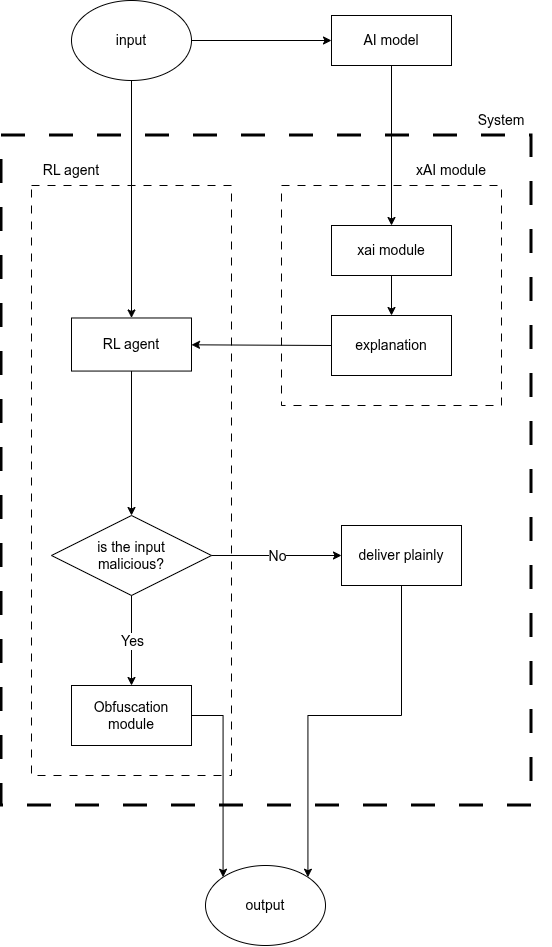
\includegraphics[width=\columnwidth]{fig1_overview.png}}
\caption{High-level overview of the system architecture.}
\label{fig1}
\end{figure}

As illustrated in Fig.~\ref{fig1}, the high-level components of the system are:
\begin{itemize}
    \item AI Model: A model hosted and served by the inference provider. In our evaluations, we utilize both Decision Tree Ensembles (XGBoost) and Deep Neural Networks (DNN) to demonstrate architectural generalizability.
    \item Input: The query submitted for processing.
    \item RL agent: Determines how much information to conceal in an explanation to limit model extraction while preserving utility. We utilize a Proximal Policy Optimization (PPO) algorithm for this agent.
    \item Obfuscation module: Intentionally obfuscates explanations to prevent attackers from learning too much about the model.
    \item XAI module: Generates baseline explanations for the outputs of the model using frameworks such as SHAP or LIME.
\end{itemize}

\begin{figure}[htbp]
\centerline{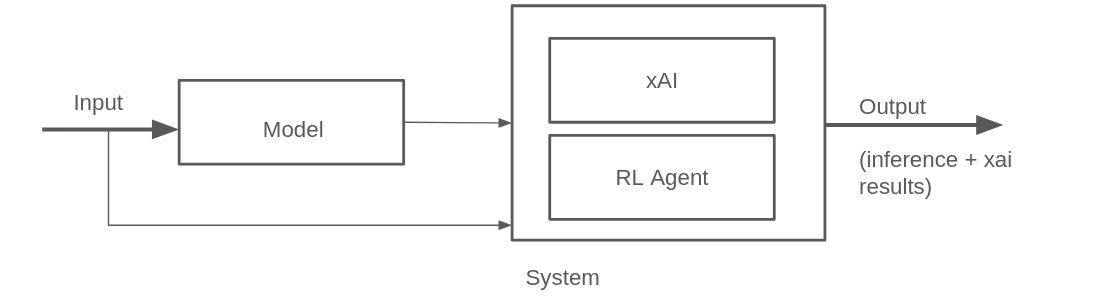
\includegraphics[width=\columnwidth]{fig2_workflow.png}}
\caption{System workflow: inference model output is explained by the XAI module and selectively obfuscated by the RL agent before returning results.}
\label{fig2}
\end{figure}

The workflow operates as follows (see Fig.~\ref{fig2}):
\begin{enumerate}
    \item An input query is submitted to the system.
    \item The input is processed on the model, generating an output.
    \item The input is simultaneously sent to the RL agent for analysis.
    \item The RL agent examines the input's relation to historical queries and determines the degree of obfuscation required.
    \item The XAI module receives the output and generates a baseline explanation, which is sent to the RL agent.
    \item The RL agent decides whether to apply obfuscation to the explanation via the obfuscation module.
    \item The processed output and the (potentially obfuscated) explanation are returned to the user.
\end{enumerate}

\section{Game Design for the RL Agent}
\subsection{Reinforcement Learning Configuration}

\textbf{Algorithm Selection:} 
To drive the dynamic obfuscation module, we employ the Proximal Policy Optimization (PPO) algorithm \cite{b23}. PPO was selected over alternative reinforcement learning algorithms, such as Deep Q-Networks (DQN) or Soft Actor-Critic (SAC), due to its inherent stability and compatibility with continuous action spaces. Because our obfuscation intensity $a_t$ is a continuous variable defined in the range $[0, 1]$, value-based methods like DQN, which require discrete action spaces, are unsuitable without arbitrary discretization. While SAC accommodates continuous actions, PPO's clipped surrogate objective function prevents destructively large policy updates, ensuring stable and monotonic improvement during the delicate min-max adversarial training process.

\textbf{State-Space Formulation and Network Architecture:} 
The RL agent must make contextual decisions based on the current query and the history of adversarial interactions. To achieve this efficiently without the computational overhead of processing full sequential arrays, the state-space $s_t$ embeds the temporal context via a history ratio. Specifically, the observation is formulated as the concatenation of the flattened current feature query $x_t$ and the normalized step counter:
\begin{equation}
s_t = \left[x_t \parallel \frac{t}{T_{max}}\right]
\end{equation}
Where $t$ is the current query step and $T_{max}$ represents the maximum allowed queries in a session. This combined vector is processed by the PPO agent, which is parameterized using a standard Multi-Layer Perceptron (MLP) architecture. The MLP network acts as both the actor, outputting the continuous action $a_t$, and the critic, estimating the state-value function to guide policy updates.

\textbf{Convergence Behavior:} 
During training, the PPO agent demonstrated robust convergence. Operating over 50,000 environmental timesteps with a learning rate of $3 \times 10^{-4}$, the agent successfully stabilized its defensive policy. Empirical learning curves derived from the environment's rolling episode rewards indicate that the agent steadily maximized its reward function, confirming that PPO effectively managed the volatile signals generated by the adversary's simultaneously evolving surrogate model.

The RL agent is trained using a game-based framework designed to enhance model security while maintaining explanation utility. The setup simulates a continuous adversarial scenario, as depicted in Fig.~\ref{fig3}.

\begin{figure}[htbp]
\centerline{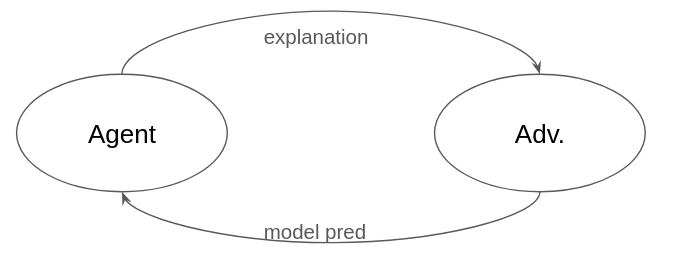
\includegraphics[width=\columnwidth]{fig3_training_loop.png}}
\caption{Game-based training loop: the RL agent obfuscates explanations; the adversary trains a surrogate model, and rewards/penalties are assigned based on security and explanation utility.}
\label{fig3}
\end{figure}

\subsection{Min-Max Game Formulation}
\textbf{Step 1: State at time $t$}\\
The state $s_{i}$ at time $t$ is the history of queries received from a specific user, where $x_{i}$ is the query and $y_{i}$ is the output.
\begin{equation}
s_i = \{(x_1, y_1), (x_2, y_2), \dots, (x_i, y_i)\}
\end{equation}

\textbf{Step 2: RL Agent Action}\\
The RL agent determines an obfuscation function $f_{obfus}$ to apply to the true explanation $E_{true}$. The action $a_t$ is a continuous variable $a_t \in [0, 1]$ representing the intensity of obfuscation. The applied transformation is defined as:
\begin{equation}
E_{output} = (1 - a_t)E_{true} + a_t \cdot \epsilon
\end{equation}
Where $\epsilon$ represents Gaussian noise scaled by the standard deviation of the true explanations ($\epsilon \sim \mathcal{N}(0, \sigma_E^2)$). If $a_t = 0$, $E_{output} = E_{true}$ (full explanation). If $a_t = 1$, $E_{output}$ relies entirely on the generated noise (full obfuscation).

\textbf{Step 3: Adversary Action}\\
The adversary leverages $E_{output}$ to construct a surrogate model $S$ targeting the original model $M$. The adversary minimizes the extraction loss $L_{extract}$:
\begin{equation}
\min L_{extract}(S(x), M(x) | E_{output})
\end{equation}

\textbf{Step 4: Reward Function}\\
The reward function $R_t$ balances security (maximizing adversary loss) and utility (minimizing explanation deviation). 
\begin{equation}
R_t = \lambda \cdot L_{extract}(S, M) - \mu \cdot ||E_{true} - E_{output}||
\end{equation}
Where $\lambda$ and $\mu$ are non-negative scalar hyperparameters weighing the importance of model security and explanation fidelity, respectively.

\section{Experimental Evaluation}
\subsection{Experimental Setup}
To evaluate the proposed methodology and demonstrate its structural generalizability, we implemented two distinct machine learning pipelines:
\begin{enumerate}
    \item \textbf{Adult Income (XGBoost + SHAP):} A black-box XGBoost target model providing interpretability via SHAP TreeExplainer.
    \item \textbf{Credit Card Fraud (DNN + LIME):} A Deep Neural Network target model providing interpretability via LIME (Local Interpretable Model-agnostic Explanations).
\end{enumerate}

In both environments, the adversary was designed as an adaptive attacker aiming to replicate the target model using a surrogate Multi-Layer Perceptron (MLP) Classifier configured with two hidden layers of 64 and 32 neurons. The RL defending agent was trained independently for each pipeline using the PPO algorithm over 50,000 timesteps.

\subsection{Evaluation Metrics}
We benchmark the defensive policies across three primary metrics to assess the balance between adversarial security and user interpretability:

\textbf{1. Average Extraction Loss ($L_{extract}$):} Measures the cross-entropy loss of the adversary's surrogate model. Higher values indicate successful defense against extraction.

\textbf{2. Average Utility Loss (L2 Distortion):} The normalized L2 norm between the true explanation and the obfuscated output, representing the raw geometric distortion.

\textbf{3. Semantic Interpretability Metrics:} To ensure the obfuscation policy does not destroy the inherent meaning of the explanations, we evaluate two semantic utility metrics:
\begin{itemize}
    \item \textit{Spearman's Rank Correlation ($\rho$):} Measures the monotonic relationship between the feature importance rankings of the original explanation $E_{true}$ and the obfuscated explanation $E_{output}$. A higher $\rho$ indicates that the relative hierarchy of feature importance is preserved.
    \item \textit{Top-$k$ Feature Agreement:} Calculates the intersection of the $k$ most critical features before and after obfuscation, defined as $\frac{|S_{true} \cap S_{output}|}{k}$, where $S$ represents the set of indices for the top $k$ features. We report results for $k=3$.
\end{itemize}

\subsection{Results and Baselines}
The trained PPO agents were benchmarked against multiple static defense strategies prevalent in the literature: Top-$k$ truncation ($k=3$), Gaussian Noise addition (level=$0.5$), Precision Reduction ($2$ decimals), and Random Subset omission ($p=0.5$). 

\begin{table*}[htbp]
\caption{Security vs. Distortion Trade-off: Adult Income Dataset (XGBoost + SHAP)}
\begin{center}
\resizebox{\textwidth}{!}{
\begin{tabular}{lcccc}
\toprule
\textbf{Strategy} & \textbf{Extraction Loss $\uparrow$} & \textbf{Utility Loss $\downarrow$} & \textbf{Spearman's $\rho$ $\uparrow$} & \textbf{Top-3 Agreement $\uparrow$} \\
\midrule
\multicolumn{5}{l}{\textit{Static Baselines}} \\
No Defense & 0.248464 & 0.000000 & 1.000000 & 1.000000 \\
Precision Reduction (2 dec) & 0.248468 & 0.006274 & 0.997749 & 0.994000 \\
Top-$k$ ($k=3$) & 0.250986 & 0.144675 & 0.941124 & 1.000000 \\
Gaussian Noise (lvl=0.5) & 0.274254 & 0.997017 & 0.611314 & 0.731333 \\
Random Subset (p=0.5) & 0.296077 & 0.603572 & 0.564830 & 0.552667 \\
\midrule
\multicolumn{5}{l}{\textit{RL Adaptive Agents ($\lambda=1.0$)}} \\
RL ($\mu \ge 0.1$) & 0.248464 & 0.000000 & 1.000000 & 1.000000 \\
\textbf{RL ($\mu = 0.05$)} & \textbf{0.257550} & \textbf{0.024615} & \textbf{0.986171} & \textbf{0.986667} \\
RL ($\mu = 0.01$) & 0.312179 & 0.845807 & 0.565143 & 0.710667 \\
RL ($\mu = 0.0$) & 0.312788 & 1.034102 & 0.469371 & 0.671333 \\
\bottomrule
\end{tabular}
}
\label{tab_adult}
\end{center}
\end{table*}

\begin{table*}[htbp]
\caption{Security vs. Distortion Trade-off: Credit Card Fraud Dataset (DNN + LIME)}
\begin{center}
\resizebox{\textwidth}{!}{
\begin{tabular}{lcccc}
\toprule
\textbf{Strategy} & \textbf{Extraction Loss $\uparrow$} & \textbf{Utility Loss $\downarrow$} & \textbf{Spearman's $\rho$ $\uparrow$} & \textbf{Top-3 Agreement $\uparrow$} \\
\midrule
\multicolumn{5}{l}{\textit{Static Baselines}} \\
No Defense & 0.991585 & 0.000000 & 1.000000 & 1.000000 \\
Precision Reduction (2 dec) & 0.983225 & 0.491624 & 0.828449 & 0.485333 \\
Top-$k$ ($k=3$) & 0.987773 & 0.770182 & 0.528731 & 1.000000 \\
Gaussian Noise (lvl=0.5) & 0.984138 & 0.662956 & 0.807614 & 0.527333 \\
Random Subset (p=0.5) & 0.985825 & 0.708359 & 0.644454 & 0.462667 \\
\midrule
\multicolumn{5}{l}{\textit{RL Adaptive Agents ($\lambda=1.0$)}} \\
RL ($\mu = 0.05$) & 0.987885 & 0.049346 & 0.977625 & 0.965333 \\
\textbf{RL ($\mu = 0.01$)} & \textbf{0.983497} & \textbf{0.130573} & \textbf{0.946349} & \textbf{0.898667} \\
RL ($\mu = 0.0$) & 0.990951 & 0.216321 & 0.915109 & 0.838667 \\
\bottomrule
\end{tabular}
}
\label{tab_credit}
\end{center}
\end{table*}

As demonstrated in Table \ref{tab_adult}, static methods struggle to balance the tradeoff effectively on the SHAP pipeline. While Gaussian Noise and Random Subset methods exhibit higher security, they inflict severe utility loss (0.997017 and 0.603572, respectively), rendering the explanations functionally useless for benign users. In contrast, the RL Agent ($\mu=0.05$) successfully increases security (0.257550) over the baseline (0.248464) while maintaining an exceptional explanation fidelity (Top-3 Agreement $\approx 0.98$).

The evaluation on the Credit Card Fraud dataset (Table \ref{tab_credit}) further demonstrates the severe limitations of static defenses when applied to LIME explanations. While Top-$k$ Truncation ($k=3$) maintains perfect Top-3 Agreement, it completely disrupts the overall feature ranking ($\rho \approx 0.52$). Conversely, Precision Reduction preserves general ranking ($\rho \approx 0.82$) but loses over half of the most critical top-3 features (Agreement $\approx 0.48$). Our adaptive policy ($\lambda=1.0, \mu=0.01$) successfully navigates this trade-off, maintaining high rank correlation ($\rho \approx 0.94$) and preserving the most critical features (Top-3 Agreement $\approx 0.89$) while defending against the extraction.

\begin{figure}
    \centering
    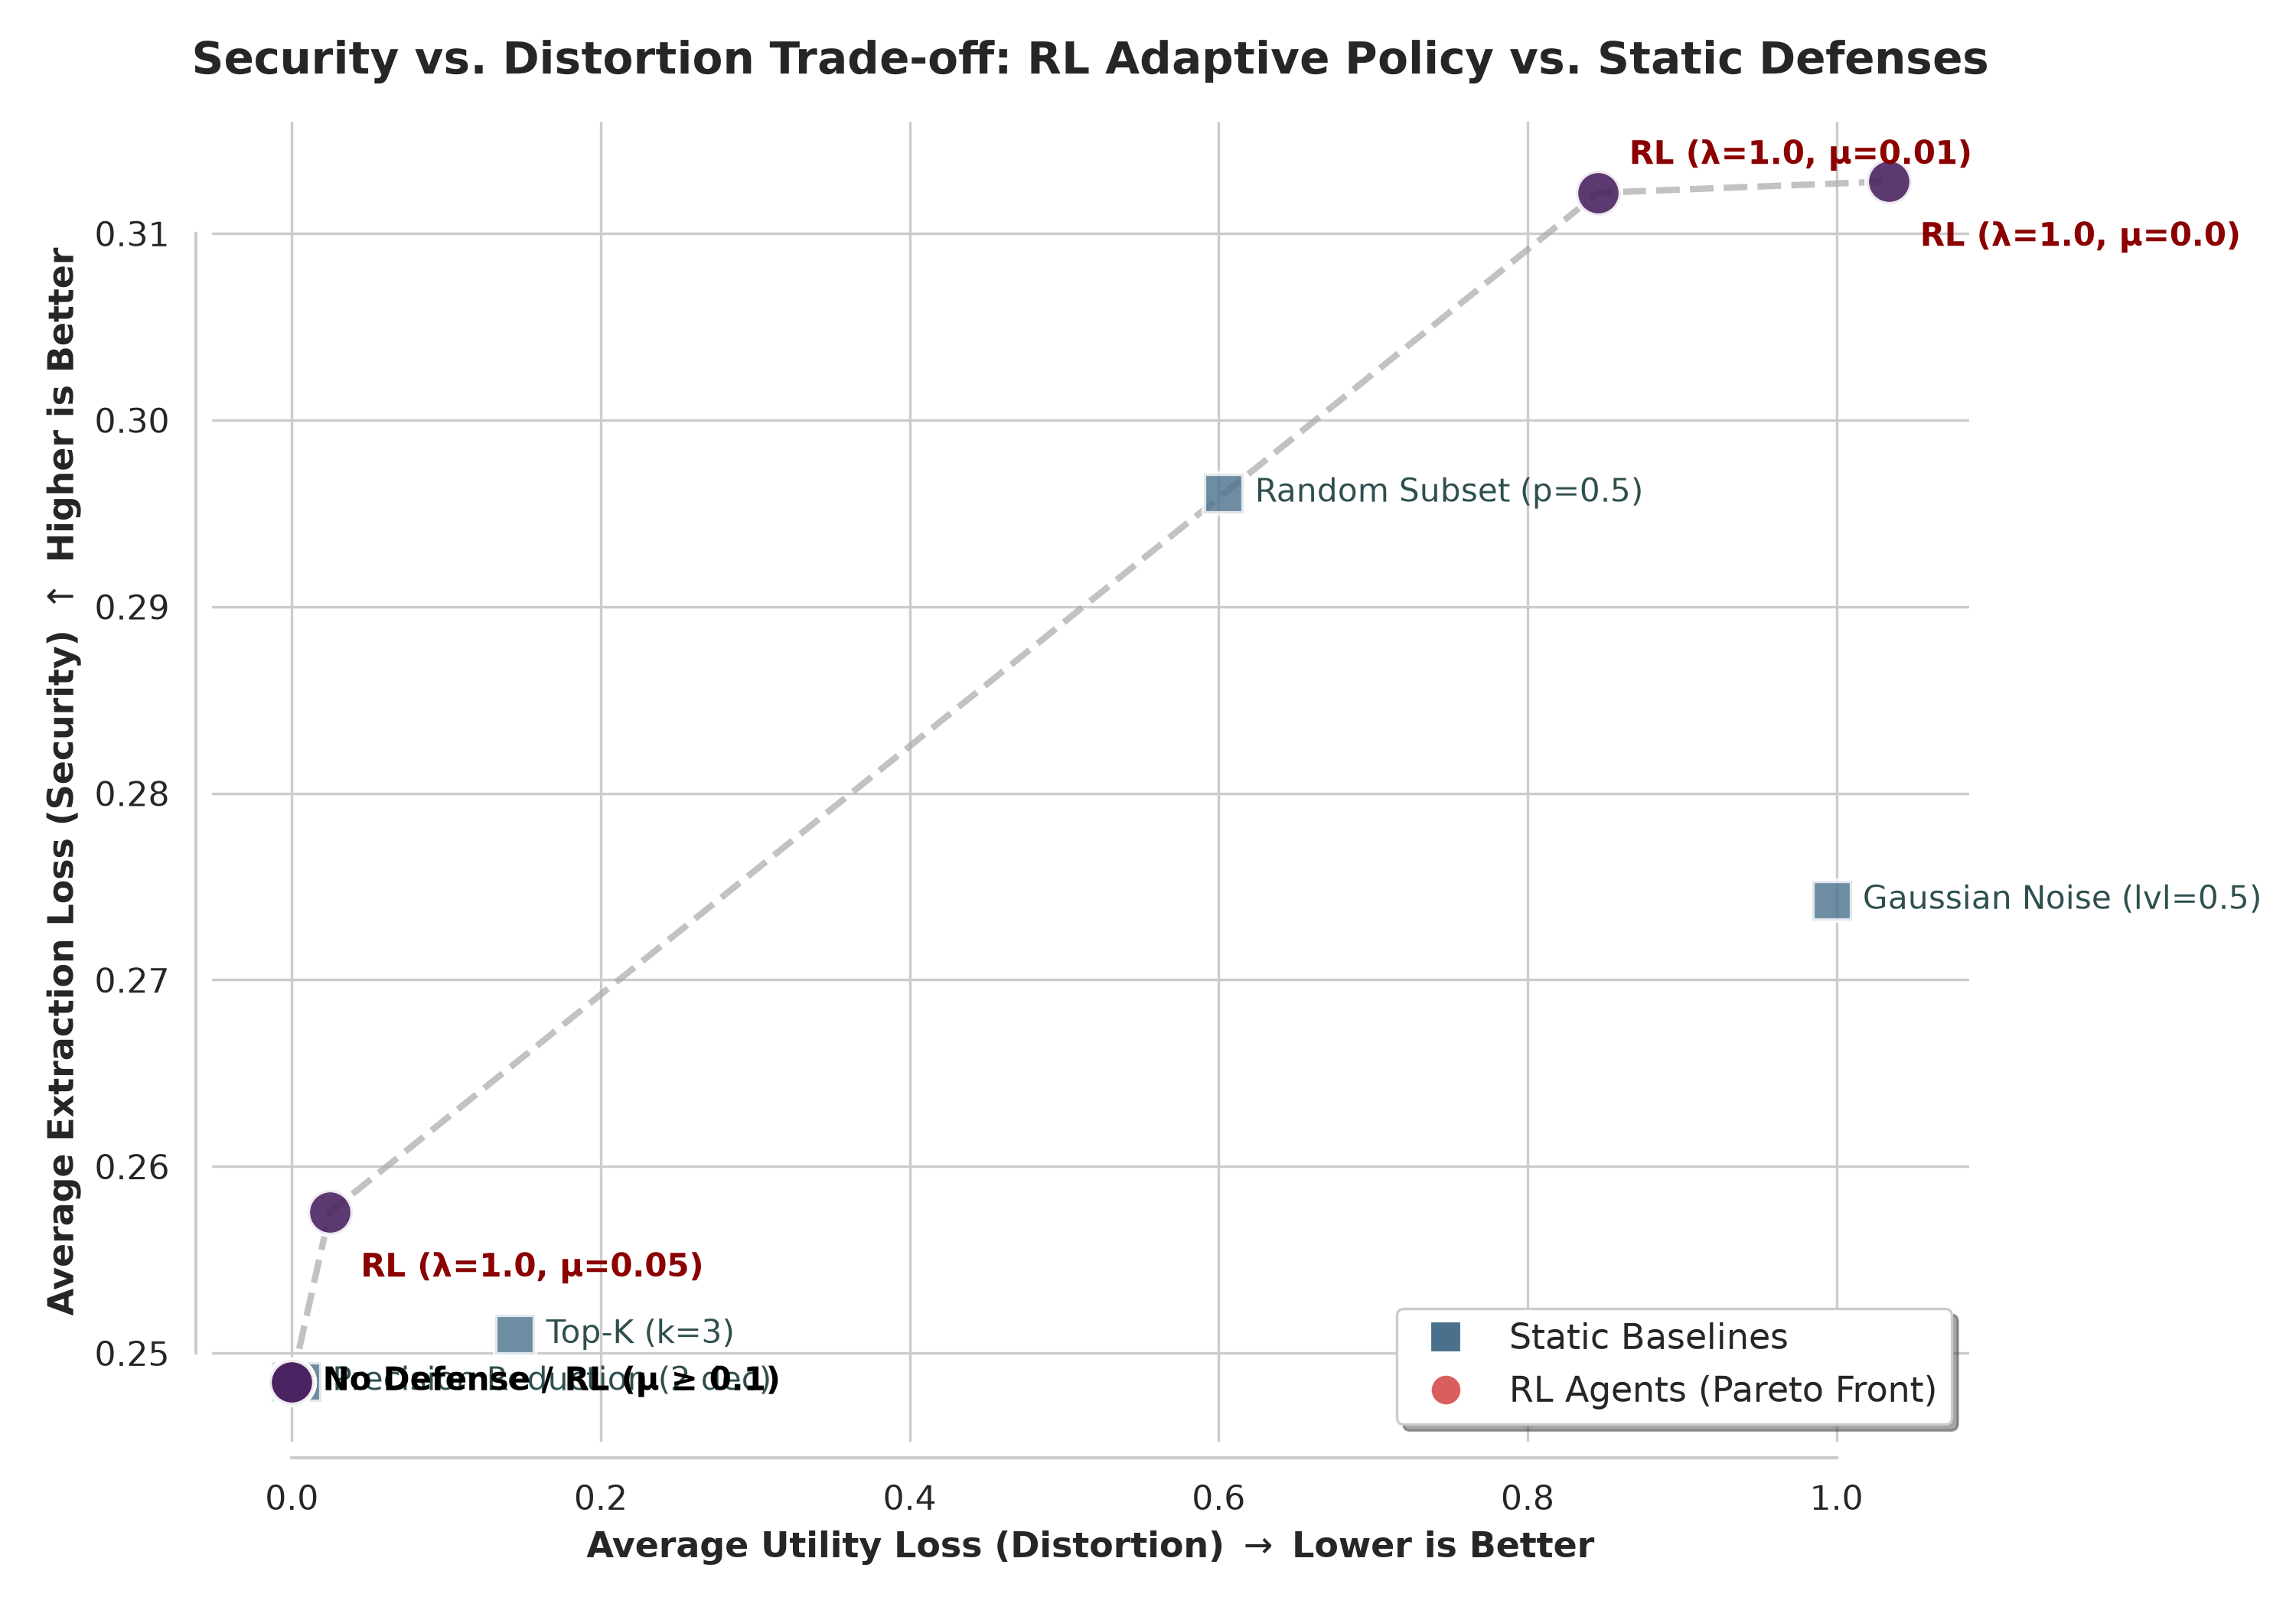
\includegraphics[width=1\linewidth]{security_vs_distortion_academic.png}
    \caption{Security versus Distortion Pareto Front}
    \label{fig_pareto}
\end{figure}

\section{Discussion and Practical Deployment}

\subsection{Addressing Computational Overhead}
A primary concern when integrating adaptive defense mechanisms into production machine learning pipelines is the introduction of unacceptable latency during real-time inference. Traditional reinforcement learning training is computationally intensive; however, the deployment phase of our proposed architecture introduces negligible overhead. 

The trained PPO actor is parameterized as a lightweight Multi-Layer Perceptron (MLP). During inference, calculating the obfuscation intensity $a_t$ requires only a single forward pass through this shallow neural network. The computational bottleneck in the proposed architecture remains the generation of the baseline XAI explanation (e.g., calculating SHAP or LIME values), not the execution of the RL defensive policy. Therefore, the dynamic obfuscation layer can be deployed as an API gateway proxy without violating strict latency service-level agreements (SLAs).

\subsection{Dynamic Threat Posturing}
The ablation study demonstrates that a single RL architecture can accommodate diverse security postures. In a practical deployment, a centralized security orchestration system could dynamically swap the active RL agent weights based on the current global threat level. During periods of normal operation, the system can utilize a high-utility agent ($\mu = 0.05$). If an intrusion detection system (IDS) flags an ongoing distributed XaMEA attack, the gateway can instantly pivot to a high-security agent ($\mu = 0.01$), actively stifling the extraction attempt while still providing baseline, albeit noisy, interpretability.

\section{Advantages of the Proposed Solution}
The dynamic integration of the RL agent provides several technical benefits:
\begin{itemize}
    \item \textbf{Enhanced Security:} Mitigates model extraction attacks by limiting explanation detail during suspicious activity.
    \item \textbf{Adaptive Explanations:} Continuously monitors query patterns and adapts the detail level based on historical interactions.
    \item \textbf{Balanced Utility:} As evidenced by the empirical benchmarks, authorized users receive high-quality insights with negligible semantic distortion, while adversaries are successfully stifled.
    \item \textbf{Robustness:} The RL agent adapts over time, effectively countering evolving attack strategies across varied architectures (Tree Ensembles and DNNs) and XAI methods (SHAP and LIME).
\end{itemize}

\section*{Acknowledgment}
The authors acknowledge the use of generative AI tools (specifically, large language models) to assist with code optimization, script debugging, and language proofreading during the preparation of this manuscript. All AI-assisted outputs were thoroughly reviewed, edited, and validated by the human authors, who take full and final responsibility for the originality, accuracy, and integrity of this work.

\bibliographystyle{IEEEtran}
\bibliography{references}


%\begin{thebibliography}{00}

%\end{thebibliography}
\end{document}